\section{Results}

Training of the models 

The resulting optimal policies are plotted in \ref{fig: Optimal policy - Infinite} for the infinite situation and \ref{fig: Optimal policy - Finite} for the finite situation.  

Optimal hyperparameters were selected for each situation via a grid-search approach, in which a selection of hyperparameters were tested and compared. These hyperparameters are indicated in respective figures. 
epsilon =0.1
gamma = 1
alpha decay = varied. 

Speak about convergence in each situation via graph

Speak about policies

\begin{figure}[ht] \label{fig: Optimal policy - Infinite} 
    \centering
    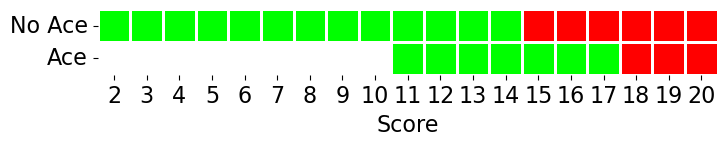
\includegraphics[width=\singlefigure]{figures/infinite_optimal_policy.png}
    \caption{Optimal policy for the infinite situation, with green indicating hit, and red indicating stick.}
\end{figure}

\begin{figure}[ht] \label{fig: Optimal policy - Finite} 
    \centering
    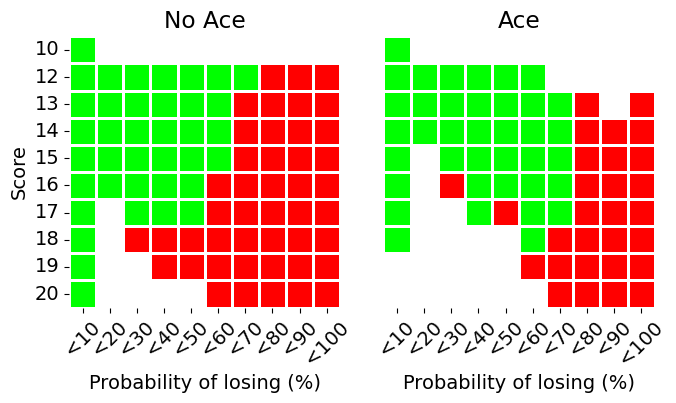
\includegraphics[width=\singlefigure]{figures/finite_optimal_policy.png}
    \caption{Optimal policy for the finite situation, with green indicating hit, and red indicating stick. Probability bins of 10\% increments are indicated accordingly.}
\end{figure}

Ideas;
* policy
* ideal policy (needs mathematical modelling)
* learning rates (and alpha rates?) : absolute and relative changes - derivatives
* differences between held ace and no held ace
* actual score (moving average?)